%%%%%%%
%  TP 8-9  %
%%%%%%%

\section*{TP 8 - 9 : Pertes de charges}
\subsection*{Comportement des fluides}
La relation générale dans le cours est
\begin{equation}
	\tau _{ij} = -p\delta _{ij}+\lambda \delta _{ij} V_{kk} +2\mu V_{ij}
\end{equation}
En faisant \textbf{l'hypotèse de Stokes} : $\lambda = -\frac{2}{3}\mu$
\begin{equation}
	\tau _{ij} = -p\delta _{ij}+2\mu (V_{ij} -\frac{1}{3} \delta_{ij}V_{kk})
\end{equation}
où $\mu$ est le coefficient de vicosité dynamique $[kg/m.s]$

\subsection*{Introduction de vitesse débitante}
\begin{center}
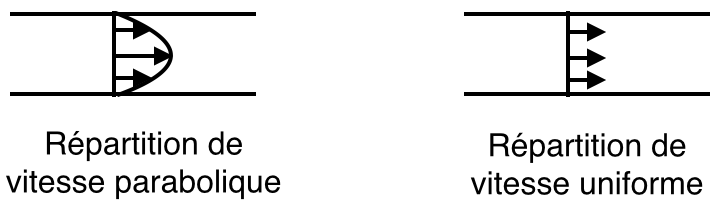
\includegraphics[scale=0.8]{rappels/tp8-1}
\end{center}

\subsection*{Bernouilli IV (le long d'un tube de courant)}
Introduisons la variation de charge $\Delta H$
\begin{equation}
	H_A = H_B + \Delta H \qquad avec \qquad H= z+\frac{P}{\rho g}+\alpha \frac{u^2}{2g}
\end{equation}
où $u$ est la vitesse débitante et $\alpha$ un coefficient qui tient compte de la répartition 
\begin{equation}
	\alpha = 
	\left\{
	\begin{aligned}
	&1 \qquad \mbox{si répartition uniforme}\\
	&2 \qquad \mbox{si répartition parabolique}
	\end{aligned}
	\right.
\end{equation}

\subsection*{Pertes de charges}
\begin{itemize}
	\item Réparties
	\begin{equation}
		\Delta H = \lambda \frac{L}{D}\frac{u^2}{2g}
	\end{equation}
	où $\lambda$ est le coefficient de perte de charge, $L$ la longeur de la conduite, $D$ son diamètre et $u$ la vitesse débitante
	
	\item Concentrées
	\begin{equation}
		\Delta H = K \frac{u^2_{ref}}{2g}
	\end{equation}
	où $K$ est le coefficient de perte de charge et $u_{ref}$ la vitesse de référence qui doit être pris comme indiqué dans le tableau ci-dessous (1 et 2 dans l'ordre de l'écoulement)
\end{itemize}	
Pour la cavitation, il faut diviser notre circuit si une pompe/turbine est présente. Etablir vite fait Bernouilli pour repérer le point de faible pression. \\

	\begin{center}
	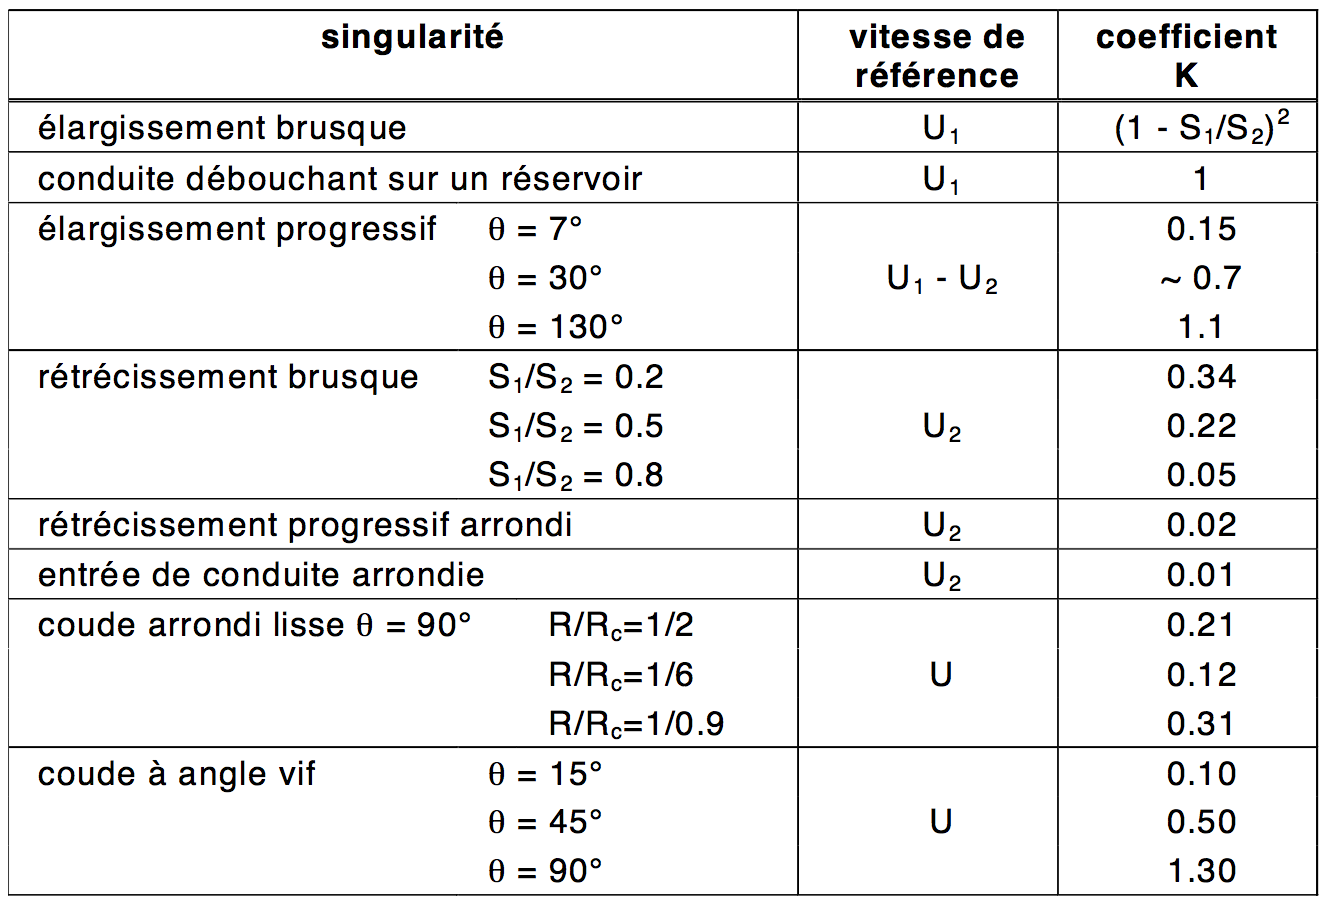
\includegraphics[scale=0.58]{rappels/tp8-2}
	\end{center}
